\documentclass[a4paper]{article} % Specify A4 paper

% Optional packages
\usepackage[utf8]{inputenc} % Allows UTF-8 input
\usepackage[T1]{fontenc}    % Selects font encodings
\usepackage{amsmath}        % For mathematical formulas
\usepackage{graphicx}       % To include images
\usepackage[ngerman]{babel} % German language support
\usepackage{geometry}       % For page layout adjustments
\usepackage{lipsum}         % For generating dummy text to fill pages
\usepackage{blindtext}      % Another package for dummy text

% Adjust page margins if needed (optional, default article margins are usually fine)
% \geometry{a4paper, margin=2.5cm}

% Document information
\title{Dokumentation zur Pipeline-Architektur}
\author{Ihr Name / Projektgruppe}
\date{\today}

\begin{document}

\section{Praktische Umsetzung: Beispiel einer Datenverarbeitungs-Pipeline}
\subsection{Gesamtarchitektur}
Um die Konzepte der Pipeline-Architektur zu verdeutlichen, ist dieser Ausarbeitung eine Beispielanwendung beigelegt. Diese Anwendung zeigt anschaulich, wie eine Pipeline aufgebaut ist und welche Vorteile sie bietet.

Abbildung \ref{fig:application_structure} illustriert den Aufbau der Demo-Anwendung. Im Bereich „Pipeline Start“ befinden sich zwei Schaltflächen: „Open“ und „Update“. Mit „Open“ wird der Pipeline-Prozess gestartet, mit „Update“ kann dieser aktualisiert werden. Im Bereich „Pipeline Config“ kann der Nutzer verschiedene Pipeline-Segmente aktivieren und deren Parameter konfigurieren, um unterschiedliche Ergebnisse zu erzielen. Die verarbeiteten Bilder werden anschließend im Bereich „Ergebnis Ausgabe“ angezeigt, sodass der Benutzer die Pipeline-Ergebnisse live verfolgen kann.

\begin{figure}[htbp]
    \centering
    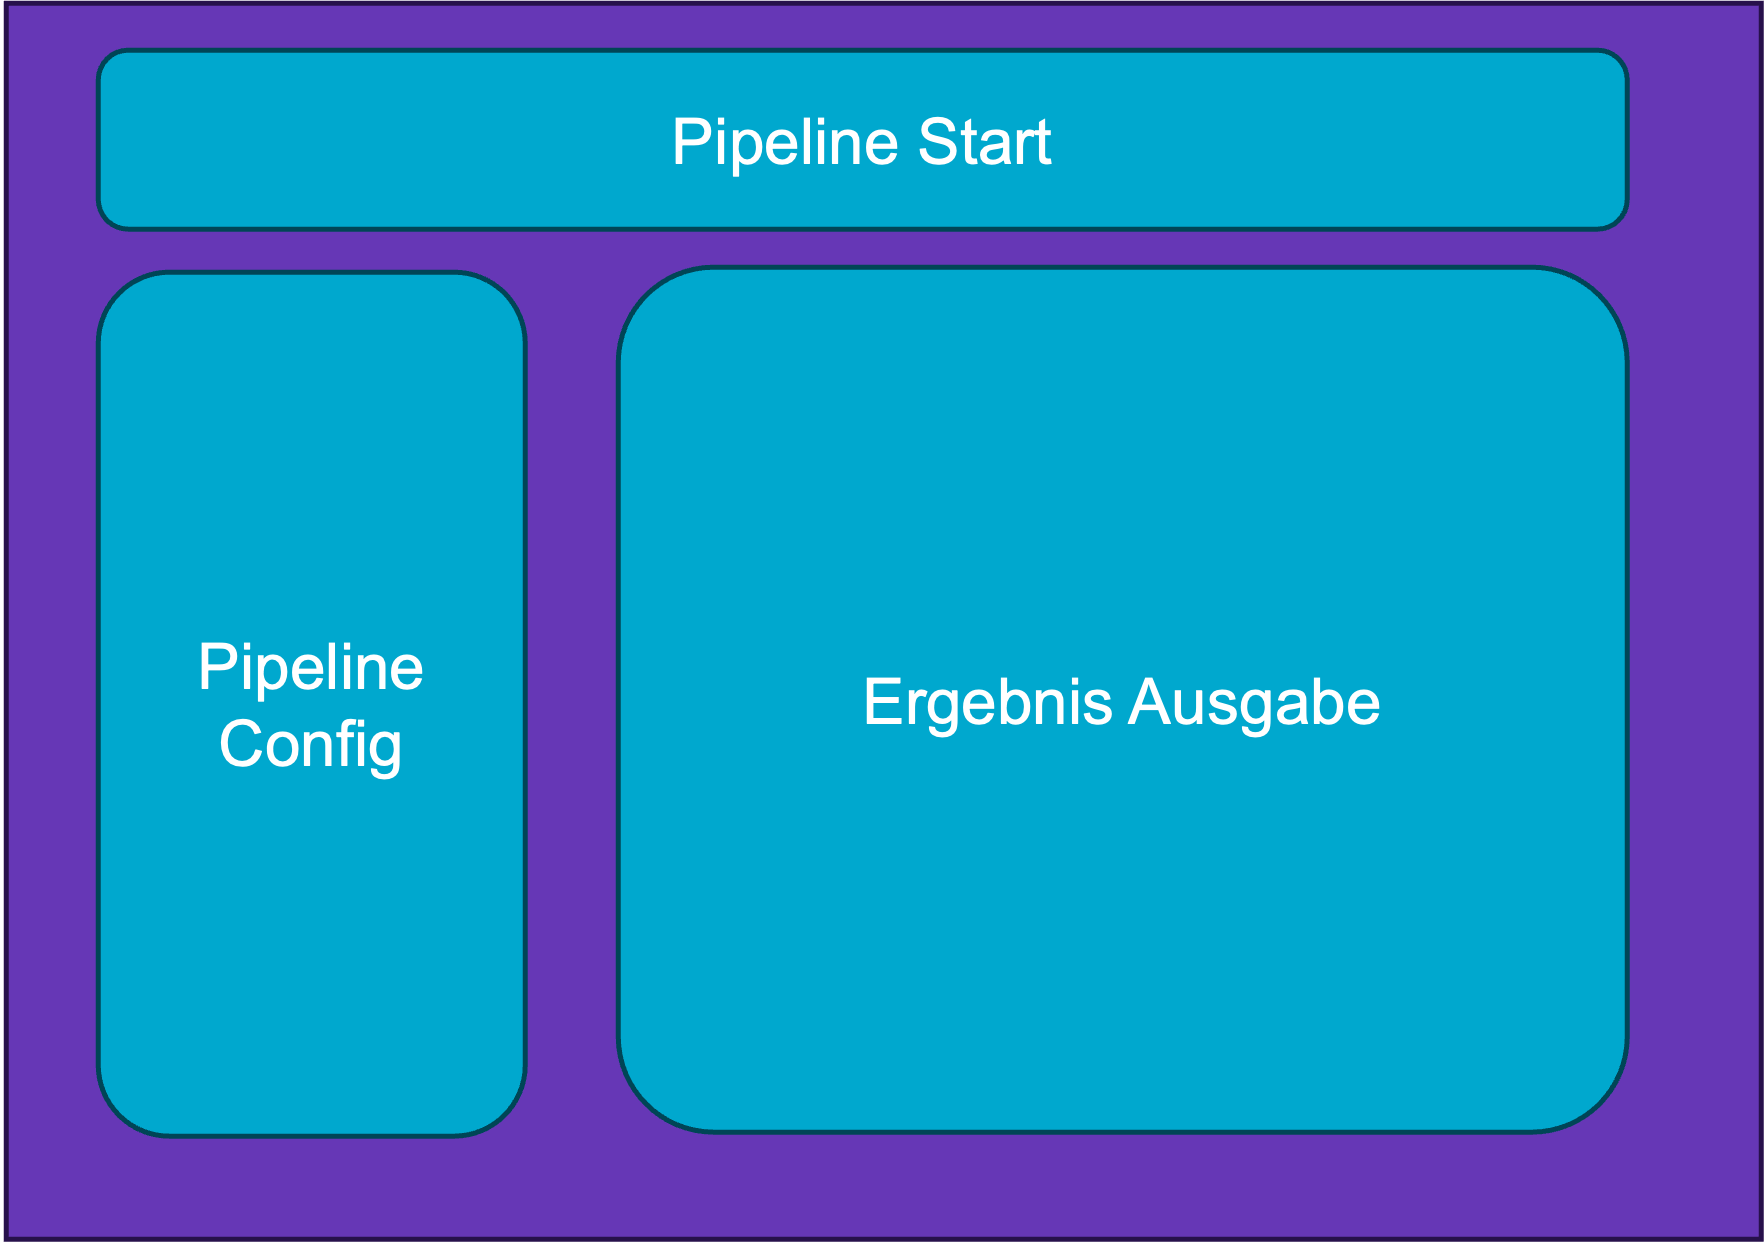
\includegraphics[width=0.5\textwidth]{img/ApplicationStructure.png}
    \caption{Aufbau der Demo-GUI.}
    \label{fig:application_structure}
\end{figure}

\begin{samepage}
Die GUI selbst ist nicht Teil der Pipeline, sondern nach dem MVC-Pattern aufgebaut. Sie nutzt lediglich die Pipeline-Architektur. Dadurch bleibt die Pipeline unabhängig von der GUI und kann auch an anderer Stelle wiederverwendet werden. Abbildung \ref{fig:gui_pipeline_interface} verdeutlicht diese Trennung: Die GUI steuert die Pipeline lediglich an und zeigt die Ergebnisse an, ohne direkt in deren Logik einzugreifen.

\begin{figure}[htbp]
    \centering
    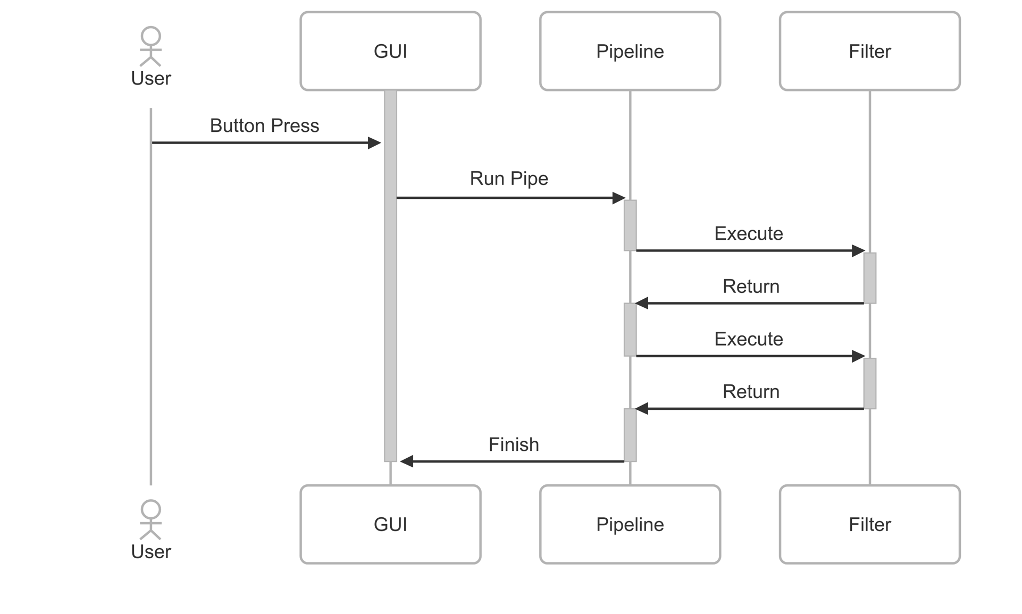
\includegraphics[width=0.7\textwidth]{img/GuiPipelineInterface.png}
    \caption{Kommunikation zwischen GUI und Pipeline.}
    \label{fig:gui_pipeline_interface}
\end{figure}
\end{samepage}

Wird die Pipeline über den „Open“-Button gestartet, öffnet sich zunächst ein Dateiauswahldialog, in dem der Benutzer die zu verarbeitende Datei auswählt. Dies ist der Einstiegspunkt in die Pipeline, die aus den folgenden Stufen besteht:

\begin{enumerate}
    \item \textbf{Loader:} In dieser ersten Stufe werden die Rohdaten von der Datenquelle (z.B. Bilddateien wie JPG, SVG etc.) eingelesen. Dazu gehört das Öffnen der Datei und das Parsen des Inhalts in eine interne Datenstruktur.
    \item \textbf{Transformer:} Auf die Daten werden Filter angewendet. Das können einfache Bildbearbeitungsschritte wie Drehen oder Spiegeln sein, aber auch komplexere Transformationen wie eine Bildanalyse mittels neuronaler Netze, um Merkmale zu extrahieren oder zu klassifizieren.
    \item \textbf{Tester:} Tester-Stufen prüfen, ob die Transformer korrekt angewendet wurden und die Ergebnisse den Erwartungen entsprechen.
    \item \textbf{Consumer:} Die verarbeiteten Ergebnisse werden gespeichert (z.B. in einer Datei oder Datenbank) oder an nachfolgende Systeme weitergegeben, etwa an die GUI zur Anzeige.
\end{enumerate}

\subsection{Implementierung der Pipeline-Steuerung: Die Wrapper-Klasse}
Die Implementierung einer Pipeline kann auf verschiedene Arten erfolgen, die sich hinsichtlich Flexibilität, Erweiterbarkeit und Entwicklungsaufwand unterscheiden. Gängige Ansätze sind:

\begin{itemize}
    \item \textbf{Direkte Implementierung im Code:} Die Reihenfolge der Stufen wird direkt im Code festgelegt. Das ist für kleine Pipelines einfach, wird aber bei wachsender Komplexität schnell unübersichtlich und schwer wartbar.
    \item \textbf{Konfigurationsbasierter Ansatz:} Die Pipeline-Struktur wird in einer externen Datei (z.B. YAML, JSON) definiert und zur Laufzeit geladen. Das bietet hohe Flexibilität und ermöglicht Anpassungen ohne Code-Änderungen, erfordert aber zusätzlichen Aufwand für das Parsen und Validieren der Konfiguration.
    \item \textbf{Wrapper-Klasse:} Eine eigene Klasse kapselt die Verwaltung der Stufen (Hinzufügen, Reihenfolge) und die Ausführung der Pipeline. Das fördert Struktur, Kapselung und Wiederverwendbarkeit.
\end{itemize}

Für die Beispielanwendung ist die Wrapper-Klasse der beste Ansatz. Sie trennt die Pipeline von der GUI, macht sie aber dennoch leicht zugänglich und ermöglicht dynamische Änderungen. Die zentrale Idee ist, eine Klasse (z.B. \texttt{Pipeline}) zu verwenden, die eine Liste von Pipeline-Stufen verwaltet. Jede Stufe wird als \texttt{Stage} bezeichnet und leitet von einer abstrakten Basisklasse ab. Dadurch muss jede konkrete Stufe die Methode \texttt{process} implementieren, was sicherstellt, dass alle Stufen einheitlich behandelt und von der Pipeline-Klasse aufgerufen werden können.

Die Wrapper-Klasse prüft zudem, dass nur gültige Stufen hinzugefügt werden. Dies geschieht durch Typ-Prüfungen, wie im folgenden Python-Codeausschnitt für die Methode \texttt{add\_stage} gezeigt:

\begin{figure}[htbp]
    \centering
    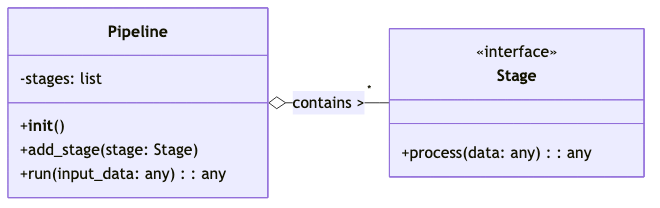
\includegraphics[width=0.8\textwidth]{img/wrapper.png}
    \caption{Klassendiagramm der Pipeline Wrapper-Klasse (\texttt{Pipeline}) und der abstrakten Stufenklasse (\texttt{Stage}).}
    \label{fig:wrapper}
\end{figure}

Damit Änderungen in einer Stage nur gezielt nachfolgende Stages beeinflussen, ist es sinnvoll, eine Datenklasse für den Datentransfer zwischen den Stages zu definieren. In der Beispielanwendung übernimmt dies die \texttt{PipeDataClass}. Jede Stage erwartet eine Instanz dieser Klasse als Parameter in der \texttt{process}-Methode und gibt eine modifizierte Instanz zurück. So bleiben die Daten zwischen den Stufen konsistent und nachvollziehbar.

Da die Demo eine Bildbearbeitung demonstriert, muss zwischen globalen und lokalen Änderungen unterschieden werden. Globale Änderungen betreffen das gesamte Bild (z.B. Drehen), während lokale Änderungen (z.B. Bounding Boxes von neuronalen Netzen oder Poster, die per Arucomarker platziert werden) nicht nachfolgende Filter beeinflussen sollen. Globale Änderungen greifen direkt auf das \texttt{base\_image\_from\_source} zu, während lokale Änderungen über \texttt{add\_optional\_layer} in eine Liste optionaler Layer eingetragen werden. Diese Layer werden in der Consumer-Stage zusammengeführt und als Ergebnis ausgegeben. Der Aufbau der \texttt{PipeDataClass} ist in Abbildung \ref{fig:pipeDataClass} dargestellt.

\begin{figure}[htbp]
    \centering
    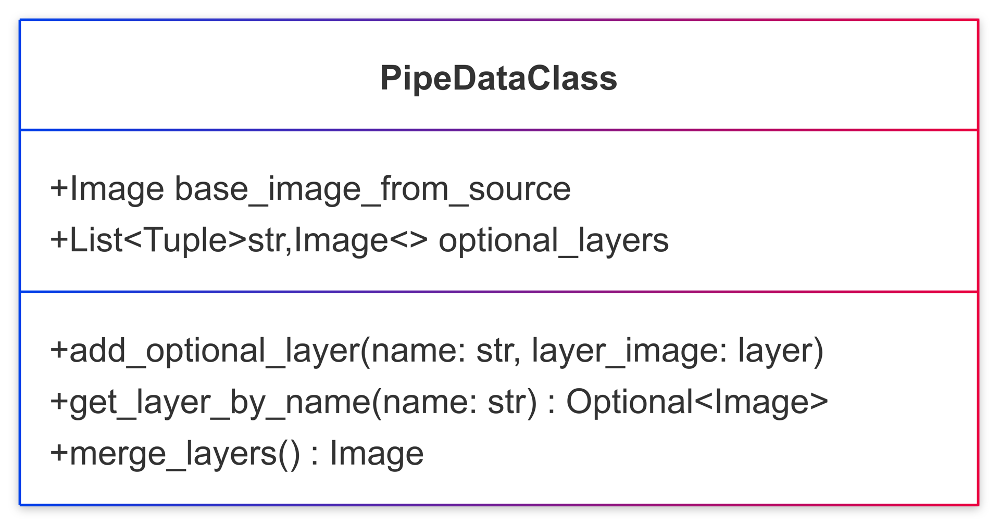
\includegraphics[width=0.8\textwidth]{img/PipeDataClass.png}
    \caption{Aufbau der PipeDataClass}
    \label{fig:pipeDataClass}
\end{figure}

\subsection{Factory Pattern zur dynamischen Komponentenauswahl}
Ein weiteres Entwurfsmuster, das die Pipeline-Architektur sinnvoll ergänzt, ist das Factory Pattern. Es dient dazu, Objekte zu erzeugen, ohne die konkrete Klasse im Voraus festlegen zu müssen. Die Verantwortung für die Objekterzeugung übernimmt eine spezialisierte Factory-Klasse oder -Methode.

Das Factory Pattern entkoppelt den aufrufenden Code von der konkreten Implementierung der zu erzeugenden Objekte. Die Factory entscheidet anhand der übergebenen Parameter oder des Kontexts, welche Unterklasse instanziiert und zurückgegeben wird.

\subsubsection{Anwendung im Datenlader}
Im Beispiel kommt das Factory Pattern beim Laden der Bilddaten zum Einsatz. Bilder liegen in unterschiedlichen Formaten vor, von pixelbasierten Formaten wie PNG und JPEG bis zu vektorbasierten wie SVG. Damit nachfolgende Stufen immer mit einheitlichen Eingangsdaten arbeiten können, erfolgt eine Transformation auf ein Standardformat (hier: pixelbasiert). Anstatt die Logik zur Erkennung und Verarbeitung jedes Formats direkt in die Pipeline-Stufe einzubauen, wird eine \texttt{LoaderFactory} verwendet.

Der Ablauf ist typischerweise wie folgt:
\begin{enumerate}
    \item Eine vorherige Pipeline-Stufe oder der Initialaufruf übergibt den Dateipfad oder eine Kennung der zu ladenden Daten an die zuständige Stufe.
    \item Diese Stufe delegiert die Erzeugung des passenden Ladeobjekts an die \texttt{LoaderFactory} und übergibt relevante Informationen (z.B. Dateipfad oder -format).
    \item Die \texttt{LoaderFactory} analysiert die Informationen (z.B. Dateiendung wie \texttt{.png} oder \texttt{.svg}).
    \item Basierend darauf instanziiert die Factory das passende Ladeobjekt (z.B. \texttt{PNG\_Loader} oder \texttt{SVG\_Loader}), das eine gemeinsame Schnittstelle (\texttt{DataLoader}) implementiert.
    \item Die Factory gibt das erzeugte Ladeobjekt an die aufrufende Pipeline-Stufe zurück.
    \item Die Pipeline-Stufe verwendet das Ladeobjekt, um die Daten zu laden, ohne die konkrete Implementierung kennen zu müssen.
\end{enumerate}

Abbildung \ref{fig:loaderFactory} zeigt diesen Entscheidungsprozess. Die Factory prüft das angeforderte Format und wählt den passenden Loader aus. Ist kein passender Loader registriert oder existiert die Datei nicht, wird ein Fehler ausgelöst oder ein Null-Objekt zurückgegeben. Für die Pipeline ist dieser Prozess transparent – der Loader verhält sich wie eine normale Stage-Klasse.

\begin{figure}[htbp]
    \centering
    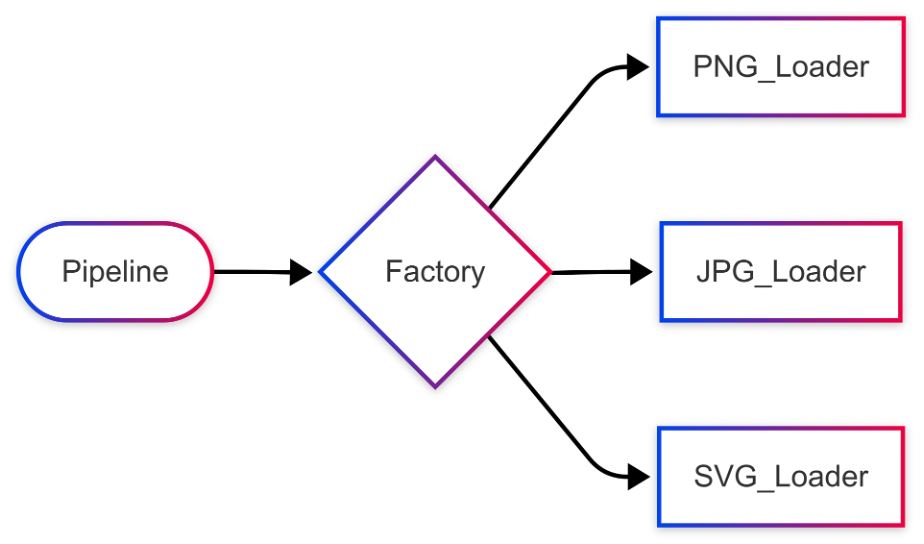
\includegraphics[width=0.8\textwidth]{img/PipelineFactory.png}
    \caption{Entscheidungsdiagramm der LoaderFactory zur Auswahl des passenden Datenladers basierend auf dem Dateiformat.}
    \label{fig:loaderFactory}
\end{figure}

\subsubsection{Vorteile des Factory Patterns in der Pipeline}
Das Factory Pattern bietet in diesem Kontext mehrere Vorteile:

\begin{itemize}
    \item \textbf{Entkoppelung:} Die Pipeline-Stufe, die Daten lädt, ist von den konkreten Ladeimplementierungen entkoppelt und arbeitet nur mit der Factory und der abstrakten Schnittstelle.
    \item \textbf{Flexibilität und Erweiterbarkeit:} Neue Dateiformate können einfach durch Implementieren einer neuen \texttt{DataLoader}-Unterklasse und Anpassen der Factory unterstützt werden, ohne die Pipeline-Stufe zu ändern.
    \item \textbf{Zentralisierung der Erzeugungslogik:} Die Entscheidung, welcher Loader wann erstellt wird, ist an einer zentralen Stelle gebündelt.
    \item \textbf{Verbesserte Testbarkeit:} Loader-Klassen und Factory können isoliert getestet werden.
    \item \textbf{Wiederverwendbarkeit:} Factory und Loader-Klassen können auch in anderen Anwendungen oder Projekten genutzt werden.
\end{itemize}

Zusammengefasst verbessert das Factory Pattern die Struktur der Pipeline, indem es die Erzeugung von Komponenten wie Datenladern flexibler, wartbarer und erweiterbarer macht.

\subsection{Pipeline mit Checkpoints}
Ein Nachteil der klassischen Pipeline-Architektur ist ihre lineare Struktur: Die Verarbeitung erfolgt in fester Reihenfolge, und es ist schwierig, den Prozess zu unterbrechen oder an einem bestimmten Punkt neu zu starten. Das kann problematisch sein, wenn Fehler auftreten oder die Verarbeitung lange dauert und der Benutzer einzelne Stufen verändern möchte.

Um dieses Problem zu lösen, können Checkpoints eingesetzt werden. Sie ermöglichen es, den Zustand der Pipeline zu einem bestimmten Zeitpunkt zu speichern, sodass die Verarbeitung später an dieser Stelle fortgesetzt oder erneut durchgeführt werden kann. Das ist besonders nützlich, wenn z.B. ein neuronales Netz ein Bild analysiert und dieser Schritt viel Zeit beansprucht.

Wie oft und an welcher Stelle Checkpoints erzeugt werden, entscheidet der Entwickler. Im Demobeispiel wird vor jeder Stage im Transformer- oder Tester-Bereich ein Checkpoint erzeugt. So kann der Benutzer jederzeit Änderungen an beliebigen Teilen der Pipeline vornehmen. Durch Drücken des Update-Buttons in der GUI (siehe Abbildung \ref{fig:gui_pipeline_interface}) wird die Pipeline an der zuletzt unveränderten Stelle neu gestartet.

\end{document}